\section{Luminosit\'a di un pianeta.}

\begin{frame}{Luce riflessa e emissione termica}

\begin{block}{luminosit\'a monocromatica (emisfero illuminato)}
\begin{align*}
&L_{\lambda,P}=A_{\lambda}\Lambda_{\lambda,P}\\
&\Lambda_{\lambda,P}=\frac{L_{\lambda}^*\pi R_P^2}{4\pi r_{P*}^2}=0.25L_{\lambda}^*\frac{R_P^2}{r_{P*}^2}\\
&L_P=\int_{Vis.}A_{\lambda}\Lambda_{\lambda,P}=A\int_{Vis}\Lambda_{\lambda,P}\,d\lambda
\end{align*}
\end{block}
\begin{block}{Manitudine visuale}
\begin{align*}
&I_V=\int_{Vis}\frac{S_V(\lambda)D_{\lambda}(\theta) L_{\lambda,P}}{4\pi r_{P,T}^2}\,d\lambda\\
&m_V=-2.5\log{I_V}+\const{}
\end{align*}
Per un pianeta molto lontano dalla stella ($r_{T*}\ll r_{P*}$)
\begin{align*}
&m_V=m_{V_0}+10\log{r_{PT}}&\intertext{$m_{V_0}$ indipendente dalla distanza.}
\end{align*}
\end{block}
\end{frame}

\begin{wordonframe}{Albedo, emissione termica, magnitudine}
Un pianeta \'e caratterizzato da emissione nel visibile e nell'infrarosso: dell'energia radiante ricevuta da un'eventuale stella parte viene riflessa e parte assorbita e riemessa nell'infrarosso.

Un pianeta di raggio $R_P$ a distanza dalla stella $r_{P*}^2$ riceve $    \Lambda_{\lambda,P}=\frac{L_{\lambda}^*\pi R_P^2}{4\pi r_{P*}^2}=0.25L_{\lambda}^*\frac{R_P^2}{r_{P*}^2}$.

se riflette una percentuale $A_{\lambda}$ (albedo). quindi per un pianeta all'opposizione si ha
\begin{align*}
&I_V=\int_{Vis}\frac{S_V(\lambda)D_{\lambda}(\theta) L_{\lambda,P}}{4\pi r_{P,T}^2}\,d\lambda=\int_{Vis}\frac{S_V(\lambda)D_{\lambda}(\theta) A_{\lambda}L_{\lambda}^*R_P^2}{14\pi^2r_{P,T}^2r_{P*}^2}\,d\lambda\\
&m_V=-2.5\log{(\int S_V(\lambda)D_{\lambda}(\theta)A_{\lambda}L_{\lambda}^*\,d\lambda)}-5\log{R_P}+5\log{r_{PT}}+5\log{r_{P*}}+\const{}\\
&=-2.5\log{(\int S_V(\lambda)D_{\lambda}(\theta)A_{\lambda}L_{\lambda}^*\,d\lambda)}-5\log{(\sqrt{A'}R_P)}+5\log{r_{PT}}+5\log{r_{P*}}+\const{}
&r_{PT}=r_{P*}-r_{T*}
\end{align*}
\end{wordonframe}

\begin{frame}{Osservazione diretta: tecniche astrometriche}
Risoluzione del sistema in maniera visuale: la separazione angolare Sole/Giove sarebbe \SI{1}{\arcsec} gi\'a a \SI{5}{\parsec}.

Estrema differenza tra $L^*$ e $L_P$: per il sistema Sole/Giove nel visibile
\begin{align*}
    \frac{L_P}{L_*}=P(\lambda,\alpha)(\frac{R_P}{a})^2\approx\num{e-9}&\intertext{$P(\lambda,\alpha)$ dipende da albedo e fase a cui si trova il pianeta.}
\end{align*}

Effetto di selezione: pianeti lontani dalla stella ($a>\SI{10}{\astronomicalunit}$).
\end{frame}

\begin{wordonframe}{Orbita stellare}
Misura posizione e moti dei corpi celesti. The path of a star orbiting star-planet barycentre appears projected on the plane of the sky as an ellipse with angular semi-major axis $\alpha$
\begin{align*}
&a_*:a_{rel}=M_p:(M_p+M_*),\ a_{rel}=a_*+a_p
&\alpha=\frac{M_p}{M_*+M_p}a\approx\frac{M_p}{M_*}a\\
&\approx(\frac{M_p}{M_*})(\frac{a}{\SI{1}{\astronomicalunit}})(\frac{d}{\SI{1}{\parsec}})\expy{-1}\si{\arcsec}
\end{align*}
Angolo sotteso da semiasse maggiore orbita ellittica stellare attorno a cm:
\begin{equation*}
\theta=\frac{m_p}{r}(\frac{P}{M_*})\expy{3/2}
\end{equation*}
P(\si{\year}), masse in masse solari e r(\si{\parsec}).
\end{wordonframe}

\subsection{Orbita del pianeta}

\begin{frame}{Moto del pianeta}
Il moto di un singolo pianeta attorno ad una stella provoca un moto riflesso della stella attorno al centro di massa. Questo provoca perturbazione delle caratteristiche osservabili
\begin{itemize}
    \item Radial velocity
    \item angular (astrometric) position in the sky
    \item arrival time of periodic reference signal 
\end{itemize}
Il pianeta e la stella orbitano attorno al comune CM in orbite ellittiche chiuse con il CM come uno dei 2 fuochi.
\begin{align*}
&r=\frac{a(1-e^2)}{1+e\cos{\nu}}\\
&\frac{x^2}{a^2}+\frac{y^2}{b^2}=1\\
&b^2=a^2(1-e^2)
\end{align*}
\begin{figure}[!ht]
\centering
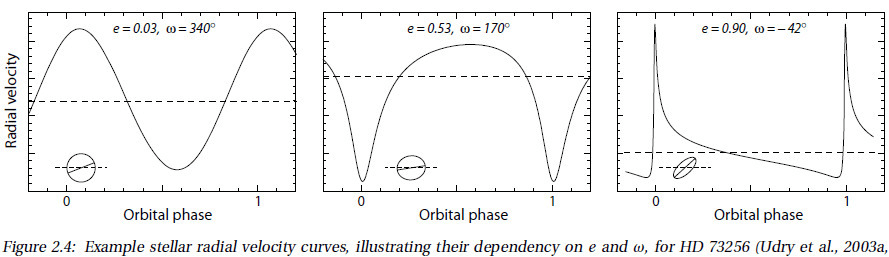
\includegraphics[width=(0.9\textwidth),height=\textheight,keepaspectratio]{vrcurve}
\caption{Stellar radial velocity curves: dependency on $e$ and $\omega$.}
\end{figure}
\end{frame}

\begin{wordonframe}{Moto del pianeta/stella attorno al CM}
Anomalia vera, $\nu(t), f(t)$: \'e l'angolo tra la direzione del pericentro e la posizione al tempo t misurata dal baricentro. L'anomalia eccentrica \'e l'angolo corrispondente all'anomalia vera riferito al cerchio ausiliario
\begin{align*}
&\cos{\nu(t)}=\frac{\cos{E(t)}-e}{1-e\cos{E(t)}}\\
&\tan{\frac{\nu(t)}{2}}=\sqrt{\frac{1+e}{1-e}}\tan{\frac{E(t)}{2}}
\end{align*}

L'anomalia medi \'e un'angolo relativo al moto medio attorno all'orbita: in un'orbita completa il pianeta non ha velocit\'a angolare costante ma una velocit\'a angolare media \'e specificata in termini del moto medio $n=\frac{2\pi}{P}$. L'anomalia media al tempo $t-t_p$ dopo il passaggio al pericentro \'e
\begin{align*}
&M(t)=\frac{2\pi}{P}(t-t_p)=n(t-t_p)\\
&M(t)=E(t)-e\sin{E(t)}
\end{align*}
\end{wordonframe}
